\documentclass{standalone}

\usepackage{tikz}
\usepackage{tkz-euclide}

\usepackage{times}

\usetikzlibrary {positioning}
\usetikzlibrary{arrows.meta}

\definecolor{accent}{rgb}{0.7,0.7,0.7}

\begin{document}
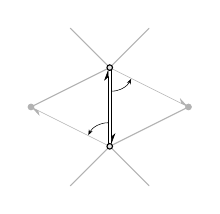
\begin{tikzpicture}[
  line/.style = {thin, color=accent},
  point/.style = {accent},
  >={Stealth[scale = 0.5]},
]

  %\tkzDefPoint(-0.5,0.0){min}
  %\tkzDefPoint(2.5,3.0){max}

  \tkzDefPoint(0.0,0.0){v0}
  \tkzDefPoint(0.0,1.0){v1}

  \tkzDefPoint(0.02,0.02){v0a}
  \tkzDefPoint(0.02,0.98){v1a}
  \tkzDefPoint(-0.02,0.02){v0b}
  \tkzDefPoint(-0.02,0.98){v1b}

  \tkzDefPoint(-0.02,0.3){v0x}
  \tkzDefPoint(0.02,0.7){v1x}

  \tkzDefPoint(-1.0,0.5){v2}
  \tkzDefPoint(1.0,0.5){v3}

  \tkzDefPoint(-0.5,-0.5){v4}
  \tkzDefPoint(0.5,-0.5){v5}

  \tkzDefPoint(-0.5,1.5){v6}
  \tkzDefPoint(0.5,1.5){v7}

  %\tkzDrawSegments(v0,v1)

  \tkzDrawSegments[line](v0,v3 v2,v1)
  \tkzDrawSegments[line](v4,v0 v0,v5)
  \tkzDrawSegments[line](v6,v1 v1,v7)

  \tkzDrawPoints[point](v2,v3)

  \tkzDrawSegments[-{Stealth[left]}](v1a,v0a v0b,v1b)
  \tkzDrawSegments[-{Stealth[left]},color=accent](v0,v2 v1,v3)
  \tkzDrawArc[color=black,->](v0b,v0x)(v2)
  \tkzDrawArc[color=black,->](v1a,v1x)(v3)

  \tkzDrawPoints(v0,v1)
  % \tkzLabelPoints(v0,v1,v2,v3,v4,v5,v6,v7)

\end{tikzpicture}
\end{document}
